% Template for NIME 2018
%
% Modified by Luke Dahl on 17 October 2-17
% Modified by Cumhur Erkut on <2016-10-11 Tue>
% Modified by Edgar Berdahl on 5 November 2014
% Modified by Baptiste Caramiaux on 25 November 2013
% Modified by Kyogu Lee on 7 October 2012
% Modified by Georg Essl on 7 November 2011
%
% Based on "sig-alternate.tex" V1.9 April 2009
% This file should be compiled with "nime-alternate.cls"


\documentclass{nime-alternate}

\begin{document}
%
% --- Author Metadata here ---
%\conferenceinfo{NIME'17,}{May 15-19, 2017, Aalborg University Copenhagen, Denmark.}
\conferenceinfo{NIME'18,}{June 3-6, 2018, Blacksburg, Virginia, USA.}

\title{DSP Filter Synthesis with Programming By Example}

%
% You need the command \numberofauthors to handle the 'placement
% and alignment' of the authors beneath the title.
%
% For aesthetic reasons, we recommend 'three authors at a time'
% i.e. three 'name/affiliation blocks' be placed beneath the title.
%
% NOTE: You are NOT restricted in how many 'rows' of
% "name/affiliations" may appear. We just ask that you restrict
% the number of 'columns' to three.
%
% Because of the available 'opening page real-estate'
% we ask you to refrain from putting more than six authors
% (two rows with three columns) beneath the article title.
% More than six makes the first-page appear very cluttered indeed.
%
% Use the \alignauthor commands to handle the names
% and affiliations for an 'aesthetic maximum' of six authors.
% Add names, affiliations, addresses for
% the seventh etc. author(s) as the argument for the
% \additionalauthors command.
% These 'additional authors' will be output/set for you
% without further effort on your part as the last section in
% the body of your article BEFORE References or any Appendices.

\numberofauthors{3} %  in this sample file, there are a *total*
% of EIGHT authors. SIX appear on the 'first-page' (for formatting
% reasons) and the remaining two appear in the \additionalauthors section.
%
\author{
% You can go ahead and credit any number of authors here,
% e.g. one 'row of three' or two rows (consisting of one row of three
% and a second row of one, two or three).
%
% The command \alignauthor (no curly braces needed) should
% precede each author name, affiliation/snail-mail address and
% e-mail address. Additionally, tag each line of
% affiliation/address with \affaddr, and tag the
% e-mail address with \email.
%
% 1st. author
\alignauthor
Mark Santolucito\\
       \affaddr{Yale University}\\
       \affaddr{51 Prospect St.}\\
       \affaddr{New Haven, CT}\\
       \email{mark.santolucito@yale.edu}
% 2nd. author
\alignauthor
Tom Murphy\\
       \affaddr{Vivid}\\
       \affaddr{P.O. Box 1212}\\
       \affaddr{Dublin, Ohio 43017-6221}\\
       \email{...}
% 3rd. author
\alignauthor Ruzica Piskac\\
       \affaddr{Yale University}\\
       \affaddr{51 Prospect St.}\\
       \affaddr{New Haven, CT}\\
       \email{ruzica.piskac@yale.edu}
}
% For your initial submission you MUST ANONYMIZE the authors.

\maketitle
%100-200 words
\begin{abstract}
Programming by example allows users to create programs without coding, by simply specifying input and output pairs.
We introduce the problem of digital signal processing programming by example, where users specify input and output wave files, and our tool can automatically synthesize a program that transforms the input to the output.
This program can then be applied to new wave files, giving users a new way to interact with music and program code.
\end{abstract}

\keywords{NIME, proceedings, \LaTeX, template}

% ------- CCS Concepts
% Here is where you enter the CCS Concepts for your paper.
%
% It is strongly recommended that authors view the submission form prior to starting to write the paper, which includes information on the CCS Concepts. 
% 
%The 2012 ACM Computing Classification System (CCS) replaces the traditional 1998 version, which has served as the de facto standard classification system for the computing field. It is being integrated into the search capabilities and visual topic displays of the ACM Digital Library. Please enter the CCS XML code for the classification terms that describe your paper. To get the XML code, please use the following procedure, which is demonstrated using three NIME-related example terms: Applied computing~Sound and music computing, Applied computing~Performing arts, and Information systems~Music retrieval.
%
% 1) Browse to the website http://dl.acm.org/ccs_flat.cfm.
% 2) Select one to three classification terms from the website that describe your paper (e.g. for the example paper Applied computing~Sound and music computing, Applied computing~Performing arts, and Information systems~Music retrieval.).
% 3) For each classification you need to select the relevance (e.g. for this example, Sound and music computing is "high", Performing arts is "low", and Music retrieval is "Medium")
% 4) Once you have selected the last term, click on "view CCS Tex Code". This will generate some code, which includes some CCSXML and some lines beginning with \ccsdesc.
% 5) Keep all of this code, as you will need it for entering into the Precision Conference System paper submission form.
% 6) For this document, keep only the \ccsdesc lines. Here is what you would paste for the classification example:

\ccsdesc[500]{Applied computing~Sound and music computing}
\ccsdesc[100]{Applied computing~Performing arts}
\ccsdesc[300]{Information systems~Music retrieval}

% this line creates the CCS Concepts section.
\printccsdesc



\section{Introduction}

There has been a proliferation of new programming languages for audio Digital Signal Processing (DSP) with languages such as SuperCollider, Faust, MaxMSP, PureData.
These languages provide a high-level interface to make DSP programming more approachable for new-comers to the field of audio programming.
DSP programming poses a particular challenge to novice programmers as writing a DSP program requires an understanding of traditional programming concepts such as loops and conditionals, as well as the ability to reason about DSP issues such as time vs frequency domain.
To assist beginning DSP programmers we turn to the Programming by Example paradigm.

Programming by Example (PBE) is a program synthesis technique that allows users to provide input and output examples to system that then automatically generates code that models the illustrated functionality.
This technique has found particular success in spreadsheets with the FlashFill tool.
In a similar vein, we hope to make DSP programming more accessible to a larger audience by using Digital Signal Processing Programming by Example (DSP-PBE).

The goal of DSP-PBE is to take an input and output audio example from the user, and synthesize the DSP program, $F$, that minimizes the distance between the transformed input, $F(i)$, and the output $o$.
In this way, a user can automatically generate the program code that captures the audio transformation demonstrated by the provided examples.
A key part of this technique is that the user receives readable DSP program code that can be further tuned or edited as the user sees fit, opening the door for learning opportunities and creative invention.


\subsection{Motivating Example}


\begin{figure}
\begin{lstlisting}
( 
SynthDef(\dsp_pbe, {|out=0|

   var main_in, id7, out6, lpf5, hpf4, psh1;
   main_in = PlayBuf.ar(2, ~buf);
   psh1 = FreqShift.ar(pitchRatio: -399.999, 
                       mul: 0.55, 
                       in: In.ar());
   hpf4 = HPF.ar(freq: 10100.0, 
                 mul: 1.562e-10, 
                 in: psh1);
   lpf5 = LPF.ar(freq: 3860.002, 
                 mul: 0.85, 
                 in: psh1);
   out6 = Mix.ar(2, [hpf4, lpf5]);
   id7 = 0.7 * out6;
   Out.ar(out, id7);

}).add;
)
\end{lstlisting}
\caption{The SuperCollider program synthesized by \ourTool to simulate the effect of a trumpet hat mute.}
\label{fig:sc_code}
\end{figure}

We demonstrate the application of \ourTool by showing how the tool is used to build a SuperCollider program that mimics the effect of a trumpet mute.
A user may want to construct a program in order to apply the effect of a trumpet mute to another sound.
To start, a user would provide an audio input example file of the trumpet without a mute (``00 none'' in Table~\ref{table:eval}), and an audio output example file (``01 hat'' in Table~\ref{table:eval}) of the trumpet playing the same note with the mute.
The user then invokes \ourTool on these two files, and the tool generates the SuperCollider program shown in Fig.~\ref{fig:sc_code}.
With this code, the user can then use the program directly in a larger SuperCollider project.
In addition, the user may wish to edit the code themselves - for example changing the mul argument to the HPF to a larger value.

In summary, this paper makes the following contributions.

\begin{enumerate}
\item We propose framework for the synthesis of DSP programs that utilize noncommutative filter types 
\item We propose an algorithm for search through the possible structural forms of a DSP filter program
\item We present our tool, \ourTool, which synthesizes SuperCollider programs from audio input/output examples, and evaluate \ourTool over a set of benchmarks
\end{enumerate}



\section{Motivating Examples}

Filter reconstruction
\begin{figure}
\centering
\begin{subfigure}{.32\linewidth}
  \centering
  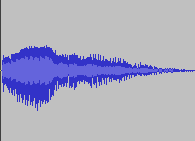
\includegraphics[width=.9\textwidth]{figs/original.png}
  \caption{Input example}
  \label{fig:inEx}
\end{subfigure}%
\begin{subfigure}{.32\linewidth}
  \centering
  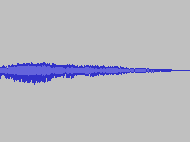
\includegraphics[width=.9\textwidth]{figs/lpf800.png}
  \caption{Output example}
  \label{fig:outEx}
\end{subfigure}
\begin{subfigure}{.32\linewidth}
  \centering
  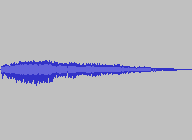
\includegraphics[width=.9\textwidth]{figs/lpf950.png}
  \caption{Generated}
  \label{fig:synthEx}
\end{subfigure}
\caption{The waveforms (a) and (b) are provided as examples, and DSP-PBE synthesizes a filter that produces (c).}
\label{fig:test}
\end{figure}

More creative applications?


\section{DSP programming by example}

The problem of DSP programming by example is formally defined as follows:
Given an input waveform $I$ and an output waveform $O$, construct a DSP filter $\synthFilter$, to minimize the aural distance $dist$ between the $O$ and $\synthFilter(I)$.
In a single line:
%
\begin{align*}
\text{Find } \synthFilter, \text{ such that } dist(O,\synthFilter(I))=0
\end{align*}


In the sequel we will describe the two key components of this statement; the definition of distance, and a search technique to find $\synthFilter$.
A distance metric that is faithful to the psycho-acoustics of the human ear is critical for a useful tool.
As an example, taking a trivial distance function that returns the difference in length of the two audio samples will allow a delay filter to satisfy any example pair of samples.

Additionally, an efficient search algorithm is critical, as the space of possible DSP filters is very large.
Not only do we need to consider a wide variety of filters, we need to consider the space of parameters for each filter, as well as the different ways of combining multiple filters.


\section{Implemention}

We used Vivid~\cite{Vivid}, a Haskell front-end for SuperCollider.

\section{Evaluation}

To evaluate our approach, we apply our synthesis algorithm to two sets of input/output examples.
The first set captures the use case of \ourTool where a user wants to model real world sounds.
This set consists of trumpet sounds with various mutes.
The second set of example input/output we run \ourTool on focuses on more creative applications.
Here we attempt to transform whitenoise into various clips from Brian Eno's Music for Airports.

The results of running \ourTool on the trumpet mute sounds benchmarks are reported in Table~\ref{table:eval}.

We need to normalize all files as the distance metric is amplitude analysis.

\begin{table}
\begin{tabular}{|l|l|c|c|c|}
\hline
\textbf{Input} & \textbf{Filter} & \textbf{dist(o, $f$(i))} & \textbf{Time (sec)}
\csvreader{results/farm.csv}{}
{\\ \hline \csvcoli & \csvcolii & \csvcoliv & \csvcolvi}
\\ \hline
\end{tabular}
\caption{Demonstrating the accuracy of the user provided refinements for the initial filter.}
\label{table:evalInit}
\end{table}

\begin{table*}[]
\begin{tabular}{|l|l|c|c|c|}
\hline
\textbf{Input} & \textbf{Output} & \textbf{dist(o, $f$(i))} & \textbf{Structural Attempts} & \textbf{Time (sec)}
\csvreader{results/trumpet.csv}{}
{\\ \hline \csvcoli & \csvcolii & \csvcoliv & \csvcolv & \csvcolvi}
\\ \hline
\end{tabular}
\caption{Evaluation on a set of benchmarks.}
\label{table:eval}
\end{table*}




%ACKNOWLEDGMENTS are optional
\section{Acknowledgments}
This work was supported by viewers like you.

%
% The following two commands are all you need in the
% initial runs of your .tex file to
% produce the bibliography for the citations in your paper.
\bibliographystyle{abbrv}
\bibliography{nime-references}  % sigproc.bib is the name of the Bibliography in this case
% You must have a proper ".bib" file
%  and remember to run:
% latex bibtex latex latex
% to resolve all references
%
% ACM needs 'a single self-contained file'!
%

%%% Place this command where you want to balance the columns on the last page. 
%\balancecolumns 

% That's all folks!
\end{document}
